\documentclass{beamer}

\mode<presentation>
{
  \usetheme{default}
  \usecolortheme{default}
  \usefonttheme{default}
  \setbeamertemplate{navigation symbols}{}
  \setbeamertemplate{caption}[numbered]
  \setbeamertemplate{footline}[page number]
  \setbeamercolor{frametitle}{fg=white}
  \setbeamercolor{footline}{fg=black}
}

\usepackage[english]{babel}
\usepackage[utf8x]{inputenc}
\usepackage{tikz}
\usepackage{listings}
\usepackage{courier}
\usepackage{array}
\usepackage{bold-extra}
\usepackage{minted}
\usepackage{fancyvrb}

\xdefinecolor{darkblue}{rgb}{0.1,0.1,0.7}
\xdefinecolor{darkgreen}{rgb}{0,0.5,0}
\xdefinecolor{darkgrey}{rgb}{0.35,0.35,0.35}
\xdefinecolor{darkorange}{rgb}{0.8,0.5,0}
\xdefinecolor{darkred}{rgb}{0.7,0,0}
\xdefinecolor{lightred}{rgb}{1,0.5,0.5}
\xdefinecolor{dianablue}{rgb}{0.18,0.24,0.31}
\definecolor{commentgreen}{rgb}{0,0.6,0}
\definecolor{stringmauve}{rgb}{0.58,0,0.82}

\lstset{ %
  backgroundcolor=\color{white},      % choose the background color
  basicstyle=\ttfamily\small,         % size of fonts used for the code
  breaklines=true,                    % automatic line breaking only at whitespace
  captionpos=b,                       % sets the caption-position to bottom
  commentstyle=\color{commentgreen},  % comment style
  escapeinside={\%*}{*)},             % if you want to add LaTeX within your code
  keywordstyle=\color{blue},          % keyword style
  stringstyle=\color{stringmauve},    % string literal style
  showstringspaces=false,
  showlines=true
}

\lstdefinelanguage{scala}{
  morekeywords={abstract,case,catch,class,def,%
    do,else,extends,false,final,finally,%
    for,if,implicit,import,match,mixin,%
    new,null,object,override,package,%
    private,protected,requires,return,sealed,%
    super,this,throw,trait,true,try,%
    type,val,var,while,with,yield},
  otherkeywords={=>,<-,<\%,<:,>:,\#,@},
  sensitive=true,
  morecomment=[l]{//},
  morecomment=[n]{/*}{*/},
  morestring=[b]",
  morestring=[b]',
  morestring=[b]"""
}

\title[2017-04-17-femtocode-diana-implementation]{Femtocode: querying HEP data}
\author{Jim Pivarski}
\institute{Princeton University -- DIANA}
\date{April 17, 2017}

\begin{document}

\logo{\pgfputat{\pgfxy(0.11, 8)}{\pgfbox[right,base]{\tikz{\filldraw[fill=dianablue, draw=none] (0 cm, 0 cm) rectangle (50 cm, 1 cm);}}}\pgfputat{\pgfxy(0.11, -0.6)}{\pgfbox[right,base]{\tikz{\filldraw[fill=dianablue, draw=none] (0 cm, 0 cm) rectangle (50 cm, 1 cm);}\includegraphics[height=0.99 cm]{diana-hep-logo.png}\tikz{\filldraw[fill=dianablue, draw=none] (0 cm, 0 cm) rectangle (4.9 cm, 1 cm);}}}}

\begin{frame}
  \titlepage
\end{frame}

\logo{\pgfputat{\pgfxy(0.11, 8)}{\pgfbox[right,base]{\tikz{\filldraw[fill=dianablue, draw=none] (0 cm, 0 cm) rectangle (50 cm, 1 cm);}\includegraphics[height=1 cm]{diana-hep-logo.png}}}}

% Uncomment these lines for an automatically generated outline.
%\begin{frame}{Outline}
%  \tableofcontents
%\end{frame}

%%%%%%%%%%%%%%%%%%%%%%%%%%%%%%%%%%%%%%%%%%%%%%%%%%%%%%%

\begin{frame}{Reminder of motivation}
\vspace{0.3 cm}
\textcolor{gray}{(The last time I presented this here was December 12.)}

\vfill
\begin{block}{\underline{Query systems}}
In some industries, it is commonplace to query petabytes of data in real time, usually with SQL. (Ibis, Impala, Kudu, Drill, etc.)
\end{block}

\vfill
\uncover<2->{For us, this would mean being able to do final analysis directly on collaboration-shared Analysis Object Datasets (AODs), without managing private skims.}

\vfill
\uncover<3->{However, these systems don't deal (well) with rich objects, like arbitrary-length lists of jets containing tracks containing hits\ldots}

\vfill
\begin{uncoverenv}<4->
\begin{block}{\underline{Femtocode}}
I'm developing a query system whose performance would permit real-time analysis, but is capable of complex manipulations, such as filtering tracks, picking pairs to compute invariant masses, etc.
\end{block}
\end{uncoverenv}
\end{frame}

\begin{frame}{Three interrelated parts}
\vspace{0.15 cm}
\begin{block}{\underline{Language/compiler}}
\vspace{-0.1 cm}
\begin{itemize}
\item As familiar as possible to the user (objects, nested loops).
\item But constrained to allow restructuring for fast execution \\ (total functions, map/filter/reduce instead of for-loops\ldots).
\item Extra-strength type system to eliminate runtime errors.
\end{itemize}
\end{block}

\vspace{-0.2 cm}
\begin{block}{\underline{Execution engine}}
\vspace{-0.1 cm}
\begin{itemize}
\item Operate on contiguous columns of data, not objects. ``Restructuring objects'' becomes changing arrays of integers.
\item No memory allocation at runtime; vectorizable loops.
\item JIT-compiled. CPU for now, but structure is right for GPU.
\end{itemize}
\end{block}

\vspace{-0.2 cm}
\begin{block}{\underline{Distributed server}}
\vspace{-0.1 cm}
\begin{itemize}
\item Vending machine: queries go in, histograms (etc.) come out.
\item Referential transparency eliminates the need of tracking users.
\end{itemize}
\end{block}
\end{frame}

\begin{frame}{}
\begin{center}
\LARGE \textcolor{darkblue}{Langauge/Compiler}
\end{center}
\end{frame}

\begin{frame}[fragile]{Start with a working example: dimuons}
\vspace{0.15 cm}
\scriptsize
\begin{Verbatim}[commandchars=\\\{\}]
pending = session.\textcolor{blue}{source}(\textcolor{red}{"ZZ_13TeV_pythia8"})
    .\textcolor{blue}{define}(\textcolor{darkgreen}{mumass} = \textcolor{red}{"0.105658"})     \textcolor{gray}{# chain of operations on source}
    .\textcolor{blue}{toPython}(\textcolor{darkgreen}{mass} = \textcolor{red}{"""}
\textcolor{red}{muons.map(mu1 => muons.map(\{mu2 =>}   \textcolor{gray}{# doubly nested loop over muons}
\textcolor{red}{  p1x = mu1.pt * cos(mu1.phi);}
\textcolor{red}{  p1y = mu1.pt * sin(mu1.phi);}       \textcolor{gray}{# shares scope with other steps}
\textcolor{red}{  p1z = mu1.pt * sinh(mu1.eta);}      \textcolor{gray}{# in the chain (see "mumass")}
\textcolor{red}{  E1 = sqrt(p1x**2 + p1y**2 + p1z**2 + mumass**2);}

\textcolor{red}{  p2x = mu2.pt * cos(mu2.phi);}
\textcolor{red}{  p2y = mu2.pt * sin(mu2.phi);}
\textcolor{red}{  p2z = mu2.pt * sinh(mu2.eta);}
\textcolor{red}{  E2 = sqrt(p2x**2 + p2y**2 + p2z**2 + mumass**2);}

\textcolor{red}{  px = p1x + p2x; py = p1y + p2y;}
\textcolor{red}{  pz = p1z + p2z; E = E1 + E2;}

\textcolor{gray}{  # "if" is required to avoid sqrt(-x)}
\textcolor{red}{  if E**2 - px**2 - py**2 - pz**2 >= 0:}
\textcolor{red}{    sqrt(E**2 - px**2 - py**2 - pz**2)}
\textcolor{red}{  else:}
\textcolor{red}{    None}   \textcolor{gray}{# output type is nullable}
\textcolor{red}{\}))}
\textcolor{red}{"""}).\textcolor{blue}{submit}()                        \textcolor{gray}{# asynchronous submission to}
final = pending.\textcolor{blue}{await}()              \textcolor{gray}{# watch result accumulate}
\end{Verbatim}

\vspace{-4 cm}
\hfill \textcolor{gray}{Yes, we see the Z peak.\hspace{0.25 cm}}

\vspace{-0.2 cm}
\hfill \mbox{\includegraphics[width=0.48\linewidth]{c1.png}\hspace{-1 cm}}
\vspace{4 cm}
\end{frame}

\begin{frame}[fragile]{Taking this example apart (1/3)}
\vspace{0.25 cm}
\begin{itemize}
\item Femtocode always appears in quotes (like SQL). It is a big-data aggregation step that feeds into a traditional analysis.

\item A query is a ``workflow'' from source to aggregation, compiled and submitted as one unit.

e.g.\ {\tt\scriptsize \textcolor{blue}{source}(\textcolor{red}{"dataset"}).\textcolor{blue}{define}(X).\textcolor{blue}{define}(Y).\textcolor{blue}{histogrammar}(Z) }

\item Most Femtocode snippets are tiny (hence ``femto''), scattered throughout a Histogrammar aggregation:

\scriptsize
\begin{Verbatim}[commandchars=\\\{\}]
session.\textcolor{blue}{source}(\textcolor{red}{"dataset"})
    .\textcolor{blue}{define}(\textcolor{darkgreen}{goodmuons} = \textcolor{red}{"""..."""})  \textcolor{gray}{# define good muons}
    .\textcolor{blue}{filter}(\textcolor{red}{"goodmuons.size >= 2"})  \textcolor{gray}{# cut on them}
    .\textcolor{blue}{define}(\textcolor{darkgreen}{dimuon} = \textcolor{red}{"""..."""}      \textcolor{gray}{# define dimuons}
    .\textcolor{blue}{bundle}(                        \textcolor{gray}{# plot their attributes}
        \textcolor{darkgreen}{mass} = \textcolor{blue}{bin}(120, 0, 12, \textcolor{red}{"dimuon.mass"}),
        \textcolor{darkgreen}{pt} = \textcolor{blue}{bin}(100, 0, 100, \textcolor{red}{"dimuon.pt"}),
        \textcolor{darkgreen}{eta} = \textcolor{blue}{bin}(100, -5, 5, \textcolor{red}{"dimuon.eta"}),
        \textcolor{darkgreen}{phi} = \textcolor{blue}{bin}(314, 0, 2*pi, \textcolor{red}{"dimuon.phi + pi"}),
                                    \textcolor{gray}{# also plot the muons}
        \textcolor{darkgreen}{muons} = \textcolor{blue}{loop}(\textcolor{red}{"goodmuons"}, \textcolor{red}{"mu"}, bundle(
            \textcolor{darkgreen}{pt} = \textcolor{blue}{bin}(100, 0, 100, \textcolor{red}{"mu.pt"}),
            \textcolor{darkgreen}{eta} = \textcolor{blue}{bin}(100, -5, 5, \textcolor{red}{"mu.eta"}),
            \textcolor{darkgreen}{phi} = \textcolor{blue}{bin}(314, -pi, pi, \textcolor{red}{"mu.phi"}))))
\end{Verbatim}
\end{itemize}
\end{frame}

\begin{frame}[fragile]{Taking this example apart (2/3)}
\vspace{0.3 cm}
\begin{itemize}\setlength{\itemsep}{0.5 cm}
\item Loop over pairs of muons is constructed by \mbox{nesting functionals:\hspace{-1 cm}}

\mbox{\tt\small \textcolor{red}{"muons.map(mu1 => muons.map(mu2 => f(mu1, mu2)))"}\hspace{-1 cm}}

is equivalent to

\begin{center}
\begin{minipage}{0.7\linewidth}
\scriptsize
\begin{minted}{python}
list_of_lists = []
for mu1 in muons:
    list_of_numbers = []
    for mu2 in muons:
        list_of_numbers.append(f(mu1, mu2))
    list_of_lists.append(list_of_numbers)

return list_of_lists
\end{minted}
\end{minipage}
\end{center}

\item There will someday be more convenient forms: \textcolor{red}{\tt pairs}, \textcolor{red}{\tt table}, \textcolor{red}{\tt filter}, \textcolor{red}{\tt flatten}, \textcolor{red}{\tt flatMap}, \textcolor{red}{\tt zip}, \textcolor{red}{\tt permutations}, etc.

\vspace{0.2 cm}
\textcolor{gray}{(The dimuon example would ideally use \textcolor{lightred}{\tt pairs} to avoid double-counting and \textcolor{lightred}{\tt flatten} to destructure the list-of-lists. Or better yet, pick two by $p_T$ to get one candidate per event.)}
\end{itemize}
\end{frame}

\begin{frame}[fragile]{Taking this example apart (3/3)}
\vspace{0.2 cm}
\begin{itemize}
\item Type system requires domain of \textcolor{red}{\tt sqrt} to be guarded:

\scriptsize
\begin{Verbatim}[commandchars=\\\{\}]
  \textcolor{red}{sqrt(E**2 - px**2 - py**2 - pz**2)}

FemtocodeError: Function "sqrt" does not accept arguments with
the given types:

    sqrt(real)

    The sqrt function can only be used on non-negative numbers.

Check line:col 19:2 (pos 401):
      sqrt(E**2 - px**2 - py**2 - pz**2)
------^
\end{Verbatim}

\vspace{0.1 cm}
\normalsize To resolve this compile-time error, we write:

\scriptsize
\begin{Verbatim}[commandchars=\\\{\}]
  \textcolor{red}{if E**2 - px**2 - py**2 - pz**2 >= 0:}
  \textcolor{red}{    sqrt(E**2 - px**2 - py**2 - pz**2)}
  \textcolor{red}{else:}
  \textcolor{red}{    None}
\end{Verbatim}

\normalsize

\item The compiler tracks each subexpression's interval of validity: \textcolor{red}{\tt\scriptsize E**2 - px**2 - py**2 - pz**2} is limited to \mbox{{\tt\scriptsize real(min=0, max=inf)}.\hspace{-1 cm}}

\vspace{0.2 cm}
In the future, we could use SymPy to discover \mbox{this algebraically.\hspace{-1 cm}}
\end{itemize}
\end{frame}

\begin{frame}{Another thing to notice}
\[
\begin{array}{ll}
\mbox{\textcolor{red}{\tt\scriptsize muons.map(mu1 => muons.map(\{mu2 =>}} & \\

\left.\renewcommand{\arraystretch}{0.7}\begin{array}{p{8 cm}}
\mbox{\textcolor{red}{\tt\scriptsize p1x = mu1.pt * cos(mu1.phi);}} \\
\mbox{\textcolor{red}{\tt\scriptsize p1y = mu1.pt * sin(mu1.phi);}} \\
\mbox{\textcolor{red}{\tt\scriptsize p1z = mu1.pt * sinh(mu1.eta);}} \\
\mbox{\textcolor{red}{\tt\scriptsize E1 = sqrt(p1x**2 + p1y**2 + p1z**2 + mumass**2);}}
\end{array}\right\} &
\mbox{only uses \textcolor{red}{\tt mu1}} \\
& \\
\left.\renewcommand{\arraystretch}{0.7}\begin{array}{p{8 cm}}
\mbox{\textcolor{red}{\tt\scriptsize p2x = mu2.pt * cos(mu2.phi);}} \\
\mbox{\textcolor{red}{\tt\scriptsize p2y = mu2.pt * sin(mu2.phi);}} \\
\mbox{\textcolor{red}{\tt\scriptsize p2z = mu2.pt * sinh(mu2.eta);}} \\
\mbox{\textcolor{red}{\tt\scriptsize E2 = sqrt(p2x**2 + p2y**2 + p2z**2 + mumass**2);}}
\end{array}\right\} &
\mbox{only uses \textcolor{red}{\tt mu2}} \\
& \\
\left.\renewcommand{\arraystretch}{0.7}\begin{array}{p{8 cm}}
\mbox{\textcolor{red}{\tt\scriptsize px = p1x + p2x;}} \\
\mbox{\textcolor{red}{\tt\scriptsize py = p1y + p2y;}} \\
\mbox{\textcolor{red}{\tt\scriptsize pz = p1z + p2z;}} \\
\mbox{\textcolor{red}{\tt\scriptsize E = E1 + E2;}} \\
\mbox{\textcolor{red}{\tt\scriptsize }} \\
\mbox{\textcolor{red}{\tt\scriptsize if E**2 - px**2 - py**2 - pz**2 >= 0:}} \\
\mbox{\textcolor{red}{\tt\scriptsize \hspace{0.25 cm}sqrt(E**2 - px**2 - py**2 - pz**2)}} \\
\mbox{\textcolor{red}{\tt\scriptsize else:}} \\
\mbox{\textcolor{red}{\tt\scriptsize \hspace{0.25 cm}None}}
\end{array}\right\} &
\mbox{uses both.} \\
\mbox{\textcolor{red}{\tt\scriptsize \}))}} & \\
\end{array}
\]
\end{frame}

\begin{frame}{Femtocode minimizes computation}
In most compilers, at least one of those two stanzas would be needlessly recomputed for every {\it pair} of muons. Physicists have learned to move these expressions out of the loop, possibly at the expense of readability.

\vfill
Femtocode's compiler turns every loop over objects into vectorized functions on individual fields. A by-product of this is that the functions depending on just \textcolor{red}{\tt mu1} or \textcolor{red}{\tt mu2} decouple from the functions depending on both.

\vfill
In fact, {\it all} duplicate subexpressions are computed exactly once. The {\it only} reason to use assignment is for clarity.

\vfill
\textcolor{gray}{(It's like an executable whiteboard.)}
\end{frame}

\begin{frame}{}
\begin{center}
\LARGE \textcolor{darkblue}{Execution engine}
\end{center}
\end{frame}

\begin{frame}[fragile]{The dimuon example, after ``compilation''}
\vspace{-0.2 cm}
\begin{columns}[t]
\column{0.5\linewidth}
\tiny
\begin{Verbatim}[commandchars=\\\{\}]
Sized by muons[]@size:
    #0       := \textcolor{red}{cos}(muons[]-phi)
    #1       := \textcolor{red}{*}(muons[]-pt, #0)
    #2       := \textcolor{red}{**}(#1, \textcolor{darkgreen}{2})
    #3       := \textcolor{red}{sin}(muons[]-phi)
    #4       := \textcolor{red}{*}(muons[]-pt, #3)
    #5       := \textcolor{red}{**}(#4, \textcolor{darkgreen}{2})
    #6       := \textcolor{red}{sinh}(muons[]-eta)
    #7       := \textcolor{red}{*}(muons[]-pt, #6)
    #8       := \textcolor{red}{**}(#7, \textcolor{darkgreen}{2})
    #9       := \textcolor{red}{+}(#2, #5, #8, \textcolor{darkgreen}{0.011164})
    #10      := \textcolor{red}{sqrt}(#9)
\textcolor{gray}{type(#10) == real(0.105658, almost(inf))}

Sized by \#11@size:
    #11@size := \textcolor{red}{$explodesize}(muons[], muons[])
    #11      := \textcolor{red}{$explodedata}(#10, #11@size, (muons[]))
    #12      := \textcolor{red}{$explodedata}(#10, #11@size, (muons[], muons[]))
    #13      := \textcolor{red}{+}(#11, #12)
    #14      := \textcolor{red}{**}(#13, \textcolor{darkgreen}{2})
    #15      := \textcolor{red}{$explodedata}(#1, #11@size, (muons[]))
    #16      := \textcolor{red}{$explodedata}(#1, #11@size, (muons[], muons[]))
    #17      := \textcolor{red}{+}(#15, #16)
    #18      := \textcolor{red}{**}(#17, \textcolor{darkgreen}{2})
    #19      := \textcolor{red}{-}(#14, #18)
    #20      := \textcolor{red}{$explodedata}(#4, #11@size, (muons[]))
    #21      := \textcolor{red}{$explodedata}(#4, #11@size, (muons[], muons[]))
    #22      := \textcolor{red}{+}(#20, #21)
    #23      := \textcolor{red}{**}(#22, \textcolor{darkgreen}{2})
    #24      := \textcolor{red}{-}(#19, #23)
    #25      := \textcolor{red}{$explodedata}(#7, #11@size, (muons[]))
    #26      := \textcolor{red}{$explodedata}(#7, #11@size, (muons[], muons[]))
\end{Verbatim}

\column{0.5\linewidth}
\tiny
\begin{Verbatim}[commandchars=\\\{\}]

    #27      := \textcolor{red}{+}(#25, #26)
    #28      := \textcolor{red}{**}(#27, \textcolor{darkgreen}{2})
    #29      := \textcolor{red}{-}(#24, #28)
    #30      := \textcolor{red}{>=}(#29, \textcolor{darkgreen}{0})
    #31      := \textcolor{red}{<}(#29, \textcolor{darkgreen}{0})
    #32      := \textcolor{red}{-}(#24, #28)
    #33      := \textcolor{red}{sqrt}(#32)
    #34      := \textcolor{red}{if}(#30, #31, #33, \textcolor{darkgreen}{None})
\textcolor{gray}{type(#34) == union(null, real(0, almost(inf)))}
\end{Verbatim}

\vspace{0.3 cm}
\hfill \fbox{\begin{minipage}{2.6 cm}
\scriptsize\raggedright {\tt muons[]-pt}, {\tt muons[]-phi}, {\tt muons[]-eta}, {\tt muons[]@size}, and everything that starts with a {\tt \#} is (at least conceptually) a big array of values.

\vspace{0.2 cm}
All functions except \textcolor{red}{\tt \$explode*} would make good GPU kernels.
\end{minipage}}
\end{columns}
\end{frame}

\begin{frame}{Freedom to choose the looping structure}
\vspace{0.2 cm}
\only<1>{\includegraphics[width=\linewidth]{dependencygraph.pdf}}
\only<2>{\includegraphics[width=\linewidth]{dependencygraph_1.pdf}}
\only<3>{\includegraphics[width=\linewidth]{dependencygraph_2.pdf}}
\only<4>{\includegraphics[width=\linewidth]{dependencygraph_3.pdf}}
\end{frame}

\begin{frame}{What are the trade-offs?}
\vspace{0.5 cm}
\begin{columns}
\column{0.4\linewidth}
Assuming the bottleneck to be memory bandwidth (usually true), \mbox{more loops:\hspace{-1 cm}}
\begin{itemize}
\item increases number of memory passes and
\item sometimes decreases number of arrays to stride simultaneously.
\end{itemize}

\vspace{0.5 cm}
Test of splitting 1 loop over 64 variables into 64 loops over 1 variable reveals a sweet spot of about 2--32.

\column{0.65\linewidth}
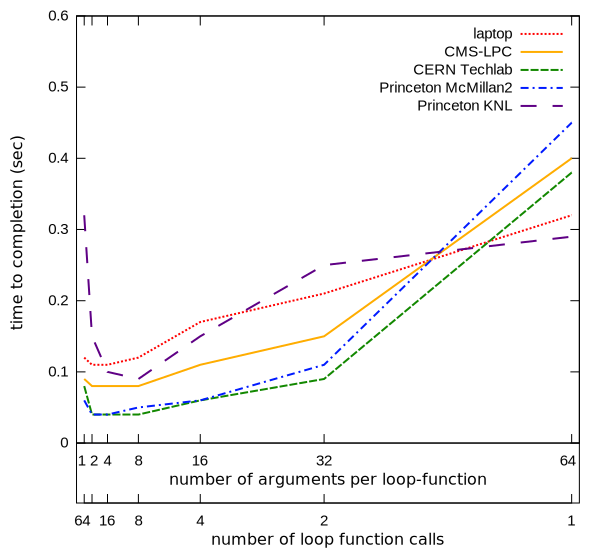
\includegraphics[width=\linewidth]{time_vs_num_arguments.pdf}
\end{columns}
\end{frame}

\begin{frame}{Sometimes you don't get to choose}
\vspace{0.3 cm}
Some vector operations have higher cardinality than others: e.g.\ a loop over jets has more steps than a loop over muons.

\vspace{0.2 cm}
Operations of different cardinality can't be in the same loop, so Femtocode divides the dependency graph into ``plateaus.''

\vspace{-0.2 cm}
\begin{center}
\only<1>{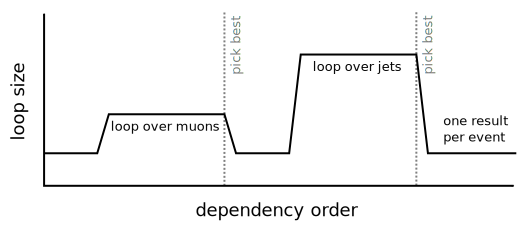
\includegraphics[width=0.8\linewidth]{plateaus1.pdf}}
\only<2->{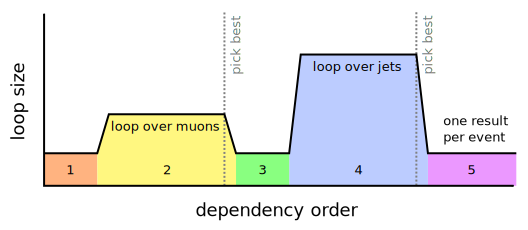
\includegraphics[width=0.8\linewidth]{plateaus2.pdf}}
\end{center}

\vspace{-0.3 cm}
\begin{uncoverenv}<2->
This cartoon example requires five loops (assuming each step strictly depends on the previous).
\end{uncoverenv}

\vspace{0.2 cm}
\begin{uncoverenv}<3->
Our dimuon example naturally splits into two loops: one over muons ({\tt\scriptsize muons[]@size}) and one over muons $\times$ muons ({\tt\scriptsize \#11@size}).
\end{uncoverenv}
\end{frame}

\begin{frame}{Three kinds of operations in each plateau}
\mbox{\hspace{-0.5 cm}\begin{minipage}{1.1\linewidth}
\begin{description}\setlength{\itemsep}{0.75 cm}
\item[Explode:] increase cardinality of one array \\ so that it matches another. \\ Determines the indexing of the \\ loop, so must be first.

\vspace{-4\baselineskip}
\hfill \includegraphics[width=0.37\linewidth]{explode.pdf}

\item[Flat:] apply function to all members of \\ two aligned data arrays, ignoring \\ event boundaries. Intermediate \\ steps need not be arrays.

\vspace{-4\baselineskip}
\hfill \includegraphics[width=0.37\linewidth]{flat.pdf}

\vspace{0.3 cm}
\item[Implode:] combine results (sum, mean, max, \\ etc.) to reduce cardinality of an \\ array. Size of output arrays are not \\ constrained by the indexing of the \\ loop. Must be last.

\vspace{-5\baselineskip}
\hfill \includegraphics[width=0.37\linewidth]{implode.pdf}
\end{description}
\end{minipage}}
\end{frame}

\begin{frame}[fragile]{Representing objects as arrays (1/2)}
\vspace{0.3 cm}
\textcolor{darkblue}{\normalsize Muon object schema:}

\scriptsize
\begin{Verbatim}[commandchars=\\\{\}]
\textcolor{darkgreen}{muons} = \textcolor{blue}{collection}(\textcolor{blue}{record}(
            \textcolor{darkgreen}{pt} = \textcolor{blue}{real}(0, almost(inf)),
            \textcolor{darkgreen}{eta} = \textcolor{blue}{real},
            \textcolor{darkgreen}{phi} = \textcolor{blue}{real}(-pi, pi)))
\end{Verbatim}

\vspace{0.3 cm}
\textcolor{darkblue}{\normalsize Physical representation:}

\scriptsize
\begin{minted}{python}
arrays_in = {
    "muons[]-pt":   [31.0960, 9.7620, 8.1769, ...,
                       5.2730, 4.7240, 8.5879],    # (length 132274)
    "muons[]-phi":  [-0.4814, -0.1242, -0.1185, ...,
                       1.2469, -0.2067, -1.7541],  # (length 132274)
    "muons[]-eta":  [0.8816, 0.9243, 0.9226, ...,
                       -0.9911, 0.9532, -0.2635],  # (length 132274)
    "muons[]@size": [7, 1, 4, ..., 4, 0, 1]}       # (length 48131)
\end{minted}

\vspace{0.3 cm}
\textcolor{darkblue}{\normalsize Dimuon run produces:}

\scriptsize
\begin{Verbatim}[commandchars=\\\{\}]
\textcolor{darkgreen}{masses} = \textcolor{blue}{collection}(\textcolor{blue}{collection}(\textcolor{blue}{union}(\textcolor{blue}{null}, \textcolor{blue}{real}(0, almost(inf)))))
\end{Verbatim}

\scriptsize
\begin{minted}{python}
arrays_out = {
    "#34":          [0.2113, 6.2386, 5.7978, ...,
                       13.1108, 0.2113, 0.2113],   # (length 584642)
    "#11@size":     [7, 7, 7, ..., 0, 1, 1]}       # (length 180405)
\end{minted}
\end{frame}

\begin{frame}{Representing objects as arrays (2/2)}
\vspace{0.3 cm}
For simple collections of records (e.g.\ particles), these arrays have the same interpretation as ROOT TLeaves:
\begin{itemize}
\item data arrays contain all values, ignoring event boundaries,
\item size array contains the size of each event's collection.
\end{itemize}

\vfill
For collections of collections (with fixed, known depth), we can extend this definition recursively:

\vspace{0.3 cm}
\textcolor{darkblue}{Given:} \hfill {\tt [} {\tt [} {\tt a} {\tt b} {\tt c} {\tt ]} {\tt [} {\tt d} {\tt e} {\tt f} {\tt g} {\tt ]} {\tt ]} {\tt [} {\tt [} {\tt h} {\tt ]} {\tt [} {\tt i} {\tt j} {\tt ]} {\tt ]}

\textcolor{darkblue}{Data array:} \hfill {\tt \ } {\tt \ } {\tt a} {\tt b} {\tt c} {\tt \ } {\tt \ } {\tt d} {\tt e} {\tt f} {\tt g} {\tt \ } {\tt \ } {\tt \ } {\tt \ } {\tt h} {\tt \ } {\tt \ } {\tt i} {\tt j} {\tt \ } {\tt \ }

\textcolor{darkblue}{Recursive counter:} \hfill \textcolor{darkorange}{\tt 2} \textcolor{blue}{\tt 3} {\tt \ } {\tt \ } {\tt \ } {\tt \ } \textcolor{blue}{\tt 4} {\tt \ } {\tt \ } {\tt \ } {\tt \ } {\tt \ } {\tt \ } \textcolor{darkorange}{\tt 2} \textcolor{blue}{\tt 1} {\tt \ } {\tt \ } \textcolor{blue}{\tt 2} {\tt \ } {\tt \ } {\tt \ } {\tt \ }

\vspace{0.3 cm}
We know whether a number in the size array refers to the size of an outer collection or an inner collection from a stack of countdowns.
\end{frame}

\begin{frame}[fragile]{Code generated for recursive counters}
\begin{center}
\scriptsize \mbox{\hspace{-1 cm}a fully general example: \textcolor{red}{\tt "xss.map(xs => xs.map(x => ys.map(y => x + y)))"}\hspace{-1 cm}}
\end{center}

\vspace{-0.5 cm}
\makebox[\linewidth]{\rule{\paperwidth}{0.3pt}}

\vspace{-0.5 cm}
\begin{columns}[t]
\column{0.5\linewidth}
\tiny
\begin{minted}{python}
entry = 0                  # entry index
deepi = 0                  # depth of collection
countdown = [0, 0, 0]      # stack of indexes
x_skip = [False, False]    # handling zero x_size
y_skip = [False]           # handling zero y_size

while entry < numEntries:  # master loop
    if deepi != 0:
        countdown[deepi - 1] -= 1

    if deepi == 0:         # xss.map(xs => ...)
        x_index[1] = x_index[0]
        countdown[deepi] = x_size[x_index[1]]
        x_index[1] += 1

        if countdown[deepi] == 0:
            x_skip[0] = True
            countdown[deepi] = 1
        else:
            x_skip[0] = False

    elif deepi == 1:       # xs.map(x => ...)
        x_index[2] = x_index[1]
        if not xskip[0]:
            countdown[deepi] = x_size[x_index[2]]
            x_index[2] += 1

        if countdown[deepi] == 0:
            x_skip[1] = True
            countdown[deepi] = 1
        else:
            x_skip[1] = False
\end{minted}
\column{0.58\linewidth}
\tiny
\begin{minted}{python}
    elif deepi == 2:       # ys.map(y => ...)
        y_index[1] = y_index[0]
        countdown[deepi] = y_size[y_index[1]]
        y_index[1] += 1

        if countdown[deepi] == 0:
            y_skip[0] = True
            countdown[deepi] = 1
        else:
            y_skip[0] = False

    elif deepi == 3:       # body of loop
        deepi -= 1

        if not x_skip[0] and not x_skip[1] \
           and not y_skip[0]:
            # put "x + y" into output array

    deepi += 1

    while deepi != 0 and countdown[deepi - 1] == 0:
        deepi -= 1         # "closing parentheses"

        if deepi == 0:
            x_index[0] = x_index[1]
            y_index[0] = y_index[1]

        elif deepi == 1:
            x_index[1] = x_index[2]

    if deepi == 0:   # master loop iterates through
        entry += 1   # deepest nesting level
\end{minted}
\end{columns}
\end{frame}

\begin{frame}{Features of the event loop}
\vspace{0.4 cm}
\begin{itemize}\setlength{\itemsep}{0.2 cm}
\item JIT-compiled for the specific nesting observed in query.
\item Never allocates memory at runtime.
\item Always two nested while-loops; the second only pops out of the stack \textcolor{gray}{(could be replaced by JIT-compiled if-statements)}.
\item Walk through data is controlled by stacks of fixed depth \mbox{\textcolor{gray}{(already replaced by JIT-compiled stack variables; 30\% speedup)}.\hspace{-1 cm}}
\item Memory access pattern is contiguous and usually forward, though it sometimes jumps backward to emulate loops like
\begin{center}
\textcolor{red}{\tt muons.map(mu1 => muons.map(mu2 => ...))}
\end{center}
\item Open question: would a version of this using recursion, rather than a single loop with stacks, be faster?
\item Generated as Python code (previous page), compiled by LLVM into native machine code. \textcolor{gray}{(Easier to test in Python.)}
\end{itemize}
\end{frame}

\begin{frame}{Why size arrays instead of runtime objects?}
\vspace{0.4 cm}
\begin{enumerate}\setlength{\itemsep}{0.2 cm}
\item To help LLVM and the hardware optimize memory bandwidth.

\vspace{0.2 cm}
\underline{Simple operation on 806177 jet $p_T$ values (6.15 MB):}

\vspace{-0.4 cm}
\begin{center}
\begin{tabular}{r l}
3 ms & no-frills loop in C \\
7 ms & Numpy's implementation \\
\textcolor{darkblue}{14 ms} & \textcolor{darkblue}{full generality Femtocode event loop} \\
24 ms & allocating C++ objects on stack and iterating \\
64 ms & allocating C++ objects on heap, iterating, deleting \\
518 ms & {\tt TTree::Draw} with {\tt TTreeCache} \\
41900 ms & CMSSW EDAnalyzer (disk access)
\end{tabular}
\end{center}

\textcolor{gray}{(Note: Femtocode should ultimately resemble the no-frills loop in C. There's work to be done.)}

\item<2-> With no event boundaries in the data arrays, the ``flat functions'' perfectly satisfy the criteria for GPU acceleration.

\vspace{0.1 cm}
\textcolor{gray}{Thus, we could automatically translate high-level code on physics objects into well-optimized GPU kernels!}
\end{enumerate}
\end{frame}

\begin{frame}[fragile]{Using ROOT functions in Femtocode}
\vspace{0.1 cm}
\tiny
\begin{minted}[frame=single]{python}
########## ROOT/some_library.py, somewhere visible to nodes on the Femtocode server.
import ctypes
libMathCore = ctypes.cdll.LoadLibrary("libMathCore.so")
chi2_ctypes = libMathCore._ZN5TMath17ChisquareQuantileEdd    # c++filt!
chi2_ctypes.argtypes = (ctypes.c_double, ctypes.c_double)
chi2_ctypes.restype = ctypes.c_double
\end{minted}

\begin{minted}[frame=single]{python}
########## Creating a custom library (on the Femtocode client):
from femtocode.typesystem import *
from femtocode.lib.custom import *

def chi2_sig(x, n):
    # Compile-time type-safety: assert parameter types, provide return type.
    assert isinstance(x, Number) and \
        almost.min(0, x.min) == 0 and almost.max(x.max, almost(1)) == almost(1)
    assert isinstance(n, Number) and n.whole and n.min > 0
    return real(0, almost(inf))

custom = CustomLibrary()            # module name          symbol name    signature
custom.add(CustomFlatFunction("chi2", "ROOT.some_library", "chi2_ctypes", chi2_sig))

########## Running a Femtocode query that uses this library:
from femtocode.run.execution import NativeTestSession
session = NativeTestSession()

# Define a dataset with the right types and fill it with dummy data.
numerical = session.source("Test", x=real(0, almost(1)), n=integer(1, almost(inf)))
for i in range(100):
    numerical.dataset.fill({"x": i / 100.0, "n": i + 1})

# Femtocode calls TMath::ChisquareQuantile without involving Python at all.
result = numerical.toPython(out = "chi2(x, n)").submit(libs=[custom])
for entry in result:
    print entry
\end{minted}
\end{frame}

\begin{frame}{}
\begin{center}
\LARGE \textcolor{darkblue}{Distributed server}
\end{center}
\end{frame}

\begin{frame}{Scaling up to full datasets}
Exploratory data analysis requires turn-around times on human timescales: seconds at most. If a query server takes much longer than this, physicists will go back to private skims.

\vfill
\textcolor{darkblue}{Scaling estimates for one query:}
\begin{itemize}
\item Typically use a dozen or so samples, totaling $\mathcal{O}(\mbox{10~TB})$.
\item Every query runs over all events, but a single query rarely uses 1\% of the {\it columns.} \textcolor{gray}{(Popularity distribution is steep.)}
\item In this early implementation of Femtocode, the worst query response times were 30~ms/MB.
\item Implies 3000 core-sec for that query: 3 seconds for 1000 cores.
\end{itemize}
\end{frame}

\begin{frame}{Scaling up to full collaborations}
\vspace{0.4 cm}
\textcolor{darkblue}{Scaling estimates for multiple users:}
\begin{itemize}
\item Most analyses have significantly overlapping needs. Evidence: home-grown skimming frameworks (Bacon, Pandas, Cms3, TreeMaker) select the same 10\% of CMS MiniAOD.
\item File I/O is more expensive than processing: $\sim$40~ms/MB versus $\sim$2~ms/MB. Everyone wins if users {\it share} cache.
\item 10\% of 10~TB of samples is 1~TB, which easily fits in RAM on a cluster of 1000 cores \textcolor{gray}{(hard to fit on one user's machine)}.
\item Short-lived queries are less likely to use resources at the same time, so shortening latency also reduces contention.
\end{itemize}

\vfill
The parameters of the final system depend on the hardware allocated for it, but improving software can steepen the performance per price.
\end{frame}

\begin{frame}{Dividing the problem}
\vspace{0.2 cm}
Femtocode's design philosophy is to do work up-front to streamline the event loop. In the distributed server, managing subtasks is part of this up-front work. Time to completion could be summarized as

\vspace{-0.2 cm}
\[
\mbox{time} = \textcolor{blue}{C_1} + \textcolor{blue}{C_2(n_{\mbox{\scriptsize cores}})} \cdot \textcolor{darkgreen}{N_{\mbox{\scriptsize subtasks}}}  + \frac{\textcolor{blue}{C_3}}{n_{\mbox{\scriptsize cores}}} \cdot \textcolor{red}{N_{\mbox{\scriptsize events}}}
\]

\vspace{-0.2 cm}
\begin{itemize}
\item \textcolor{blue}{$C_1$} is a constant, dominated by 70~ms of JIT-compilation time,
\item \textcolor{blue}{$C_2(n_{\mbox{\scriptsize cores}})$} is the time spent managing subtasks, a complex concurrent processes affected by Amdahl's law.
\item \textcolor{blue}{$C_3$} is the compiled and embarrassingly parallel part that executes the user's query.
\end{itemize}

The order parameter in this problem is $\textcolor{red}{N_{\mbox{\scriptsize events}}}$. We get to choose $\textcolor{darkgreen}{N_{\mbox{\scriptsize subtasks}}} / \textcolor{red}{N_{\mbox{\scriptsize events}}}$ and can simply make partitions larger if the Pythonic ``data management'' part becomes an issue.
\end{frame}

\begin{frame}{Distributed system layout: as implemented}
\vspace{0.15 cm}
\mbox{\hspace{-1.1 cm}\includegraphics[width=1.2\linewidth]{distributed-system-tall.pdf}}
\end{frame}

\begin{frame}{Not a batch system}
\vspace{0.5 cm}
Although incoming jobs are scattered to compute nodes, computed in parallel, and then gathered, this differs from a batch system in important ways.

\begin{enumerate}
\item \textcolor{darkblue}{No ``job id'' or attempt to send results back to the user.}

\vspace{0.1 cm}
Identical queries on the same dataset will always yield identical results, so jobs are identified by a hash of the query itself.

\vspace{0.1 cm}
Client polls for updates and may break/reestablish connection before it's done. Dispatch checks the ``store'' for partial results, rather than re-running.

\vspace{0.1 cm}
Therefore, when users refresh their analysis scripts or run tutorial examples, they don't stress the computation engine.

\item \textcolor{darkblue}{Subtasks are assigned to ``compute'' nodes according to a hash function on required input data.} Subtasks requiring the same input data go to the same nodes and are more likely to find it in cache.
\end{enumerate}
\end{frame}

\begin{frame}{Loosely coupled, resistant to failure}
Each circle on the diagram is a collection of identical nodes, none of which are single points of failure.

\begin{itemize}
\item If a ``compute'' node disappears, the hash-assignment function has a series of fallbacks.
\item The ``dispatch'' nodes are stateless; they can be load-balanced.
\item Only the ``store'' persistently holds results; it's a MongoDB instance with appropriate partitioning and replication.
\item The datasets in ``metadb'' and ``datadb'' are treated as immutable artifacts. New datasets may be created (with version numbers), but not changed in-place.
\end{itemize}
\end{frame}

\begin{frame}{}
\begin{center}
\LARGE \textcolor{darkblue}{Conclusions}
\end{center}
\end{frame}

\begin{frame}{Conclusions}

Progress on three aspects of the Femtocode query server project: getting ``above water.''

\begin{itemize}
\item \textcolor{darkblue}{Langauge/Compiler:} starting to compute meaningful quantities. Parser and type-checker are mature.
\item \textcolor{darkblue}{Execution engine:} problem of how to compute general ``explosions'' is under control. Compiling with LLVM and even serializing functions for remote execution. Factors of several from optimal performance.
\item \textcolor{darkblue}{Distributed server:} working prototype passes data through components, returns results as it should. Have not attempted to scale up.
\end{itemize}

Mature enough that there may be subprojects to split off. Ask me if you're interested!
\end{frame}

\end{document}






%% \scriptsize
%% \begin{columns}
%% \column{0.6\linewidth}
%% \begin{itemize}
%% \item {\bf client:} installed on user's machine.
%% \item {\bf dispatch:} gateway URL, checks for results and assigns if needed.
%% \item {\bf metaDB:} dataset descriptions, schemas.
%% \end{itemize}
%% \column{0.6\linewidth}
%% \begin{itemize}
%% \item {\bf compute:} runs execution engine.
%% \item {\bf dataDB:} source of data, such as EOS/XRootD or blob store.
%% \item {\bf store:} stores partial results for {\bf dispatch}.
%% \end{itemize}
%% \end{columns}
%% \begin{frame}{Story of a query}
%% \hfill \includegraphics[width=0.5\linewidth]{distributed-system-short.pdf}
%% \begin{enumerate}
%% \item {\bf Client} Femtocode-compiles a query into vectorized statements and sends it to the only exposed URL: {\bf dispatch}.
%% \item {\bf Dispatch} checks to see if there's a result in the {\bf store}; if not, it splits the job and distributes it among {\bf compute} nodes.
%% \item {\bf Compute} runs the Femtocode execution engine, executing subtasks on a first {\it ready}, first serve basis.
%% \item {\bf DataDB} is the input data from the experiments, may be EOS/XRootD. {\bf Compute} nodes cache as much input data as possible to avoid making requests to {\bf dataDB}.
%% \item {\bf Store} holds results from {\bf compute} so that {\bf dispatch} (or {\bf client}) do not need to stay alive and stateful to receive them.
%% \item {\bf MetaDB} holds dataset descriptions and schemas. May be a part of {\bf dataDB}.
%% \end{enumerate}
%% \end{frame}
